%!TEX root = ../template.tex %
% !TeX spellcheck = en_US
%%%%%%%%%%%%%%%%%%%%%%%%%%%%%%%%%%%%%%%%%%%%%%%%%%%%%%%%%%%%%%%%%%%%
%% chapter4.tex
%% NOVA thesis document file
%%
%% Chapter with lots of dummy text
%%%%%%%%%%%%%%%%%%%%%%%%%%%%%%%%%%%%%%%%%%%%%%%%%%%%%%%%%%%%%%%%%%%%

\typeout{NT FILE chapter5.tex}%

\chapter{Optical Properties of Nanostructured hBN}
\label{ch:Optical_hBN_superlattice}

In previous chapters we studied the phenomenology and technical aspects of the exciton formation, and the optical response they confer to \bd~materials, and finally the behavior of light when the exciton hybridizes with the photon, i.e., exciton-polaritons.
In this chapter we are interested as well in exciton-polaritons, but now for a \gls{hbn} monolayer with a periodic potential on top.
We have seen previously the formation of a superlattice upon applying a 2D periodic potential with square symmetry on top of a tight-binding model in a square lattice, to which we called the gapped \gls{soc} model.

Herein, we apply a 1D potential, leading to a 1D superlattice.
In this case, it is possible to obtain an analytical expression for the renormalized Hamiltonian, without resorting to perturbation theory, as we did for the case of the \gls{soc} model.
Since we have an analytical expression for the low-energy Hamiltonian, we can extract the effective masses analytically, which speeds up the process of obtaining the binding energies of the excitons.
However, due to the fact that the potential is one dimensional, we introduce a degree of anisotropy on the dispersion which depends on the periodicity and amplitude of the potential.

As the method of the \gls{bse} introduced before applies only to isotropic systems, we use instead the variational method, as we did in the case of the \gls{soc} model.
The \gls{bse} method can be extended to anisotropic systems, but is computationally more costly.
The variational method offers also the advantage of obtaining an analytical expression for the optical conductivity, apart from a final angular integral that can only be performed analytically.
With the optical conductivity, we can compute the dispersion relation of the exciton-polaritons, just like we did for the monolayer \gls{hbn}.

We divide this chapter in three parts (eventually more...).
First, we derive the expression for the renormalized low-energy Hamiltonian and discuss the new emergent electronic structure.
Next, we focus on solving the excitonic problem, that is, finding the excitonic binding energies and wavefunctions.
Afterwards, we get to focus on the optical conductivity.
We finish the chapter with the dispersion relations for the exciton-polaritons.
Throughout the chapter, we stress the difficulties introduced by potential and consequent anisotropy introduced in the dispersion along our reasoning.



\section{Nanostructured hBN: a 1D Superlattice}
\label{sec:nanostructured_hBN}

Introduces the system, also with the figure.

\begin{figure}[t]
    \centering
    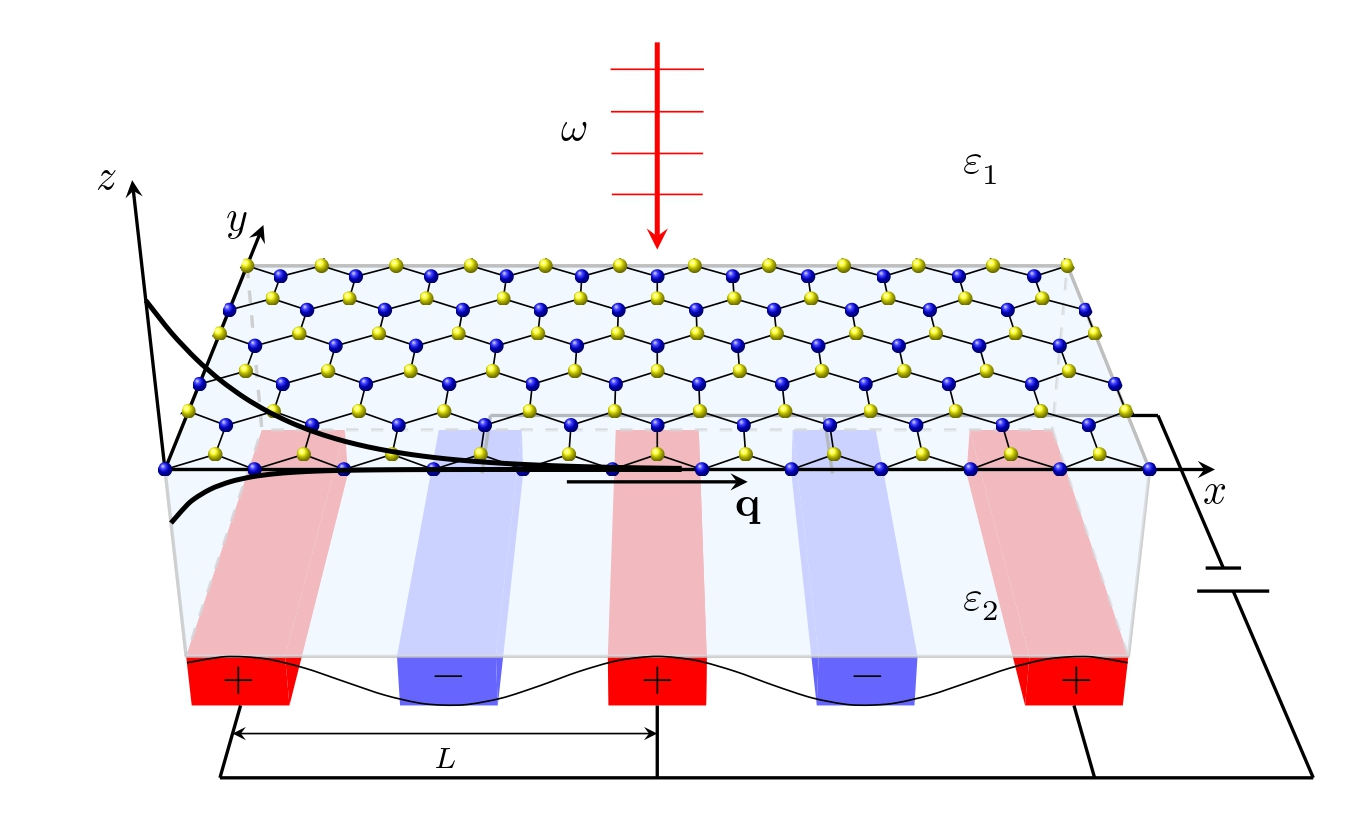
\includegraphics[width=1.\textwidth]{Chapters/Figures/Chapter_5/hBN_superlattice}
    \caption{A hBN monolayer over a substrate, subjected to an external periodic potential with period $L$ along the $x$-direction, under a time-periodic drive of a linearly polarized optical field. (b) Brillouin zone (BZ) of the original monolayer hBN, and (c) the BZ of the superlattice resulting from applying the 1D potential of (a).}
    \label{fig:hBN_monolayer}
\end{figure}


\section{Electronic Band Structure of 1D Modulated hBN}
\label{sec:electronic_band_structure_modulated_hBN}

We start from the low-energy Hamiltonian for hBN around point $K$
of the Brillouin Zone (BZ)
\begin{equation}
    H_{0}=\hbar v_{F}\mathbf{p}\cdot\boldsymbol{\sigma}+M\sigma_{z}=-i\hbar v_{F}\left(\frac{\partial}{\partial x}\sigma_{x}+\frac{\partial}{\partial y}\sigma_{y}\right)+M\sigma_{z}.
\end{equation}

Now we include a periodic potential $V(x)=V\left(x+L\right)$, with
$L\gg a$ and $a$ the atomic lattice spacing:

\begin{equation}
    H=H_{0}+V(x),
\end{equation}

with the 2 by 2 identity matrix implicit.
The potential term can be removed by introducing the unitary transformation

\begin{equation}
    U_{\alpha}=\frac{1}{\sqrt{2}}\left(
    \begin{array}{cc}
       e^{-i\alpha(x)/2} & -e^{i\alpha(x)/2}\\
       e^{-i\alpha(x)/2} & e^{i\alpha(x)/2}
    \end{array}\right),
\end{equation}

where
\begin{equation}
    \alpha(x)=\frac{2}{\hbar v_{F}}\int_{0}^{x}dx^{\prime}V(x^{\prime}).
\end{equation}

Applying this transformation to the Hamiltonian we obtain

\begin{equation}
    \bar{H}=U_{\alpha}^{\dagger}[H_{0}+V(x)]U_{\alpha}=U_{\alpha}^{\dagger}H_{0}U_{\alpha}+V(x).\label{eq:transformed_H}
\end{equation}

Now we need to simplify the term in $H_{0}$ that reads
\begin{equation}
    U_{\alpha}^{\dagger}H_{0}U_{\alpha}=\hbar v_{F}\left[U_{\alpha}^{\dagger}\sigma_{x}\frac{\partial}{\partial x}U_{\alpha}+U_{\alpha}^{\dagger}\sigma_{y}U_{\alpha}\frac{\partial}{\partial y}\right]+MU_{\alpha}^{\dagger}\sigma_{z}U_{\alpha}.\label{eq:transformed_H0}
\end{equation}

The term in $\sigma_{z}$ is the simplest and evaluates to
\begin{equation}
    MU_{\alpha}^{\dagger}\sigma_{z}U_{\alpha}=\left(\begin{array}{cc}
                                                        0 & -Me^{i\alpha}\\
                                                        -Me^{-i\alpha} & 0
    \end{array}\right).
\end{equation}

For the term involving the derivative in order to $y$, we evaluate
the matrix element between two arbitrary wavefunctions in real-space,
that, in the end, turn out to be the basis functions. We write
\[
    \begin{aligned}H_{y}[\varphi_{i},\varphi_{j}] & =\int dxdy\varphi_{i}^{\ast}(\mathbf{r})\hbar v_{F}U_{\alpha}^{\dagger}\sigma_{y}U_{\alpha}\frac{\partial\varphi_{j}(\mathbf{r})}{\partial y} = \frac{1}{2}\int dx\varphi_{i}^{\ast}(\mathbf{r})
    \left(\begin{array}{cc}
              0 & -e^{i\alpha(x)}\hbar v_{F}\\
              e^{-i\alpha(x)}\hbar v_{F} & 0
    \end{array}\right)\frac{\partial\varphi_{j}(\mathbf{r})}{\partial y} - \\
    & - \frac{1}{2}\int dx\frac{\partial\varphi_{i}^{\ast}(\mathbf{r})}{\partial y}\left(\begin{array}{cc}
                                                                                             0 & -e^{i\alpha(x)}\hbar v_{F}\\
                                                                                             e^{-i\alpha(x)}\hbar v_{F} & 0
    \end{array}\right)\varphi_{i}(\mathbf{r})
    \end{aligned}
\]

\section{Anisotropic Excitonic States}
\label{sec:anisotropic_exciton_states}

Solves Wannier equation with the variational method.

\section{Excitonic Optical Response and Absorption Spectrum}
\label{sec:exciton_optical_response}

Computes the optical conductivity and absorption (transmission and reflection) spectrum with the Fresnel coefficients.

\section{Exciton-polaritons in Modulated hBN}
\label{sec:exciton_polaritons}